\documentclass[tikz,border=4pt]{standalone}
\usepackage{amsmath}
\begin{document}
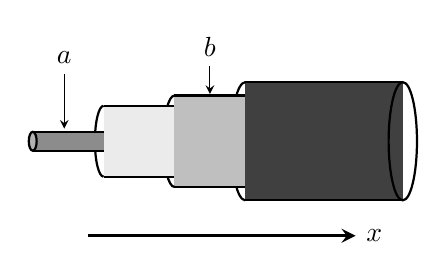
\begin{tikzpicture}[>=stealth, thick, scale=1.0]
  % Outer protective jacket (dark gray)
  \fill[black!75] (2.2, -0.75) rectangle (4.2, 0.75);
  \draw[thick] (2.2, -0.75) -- (4.2, -0.75) (2.2, 0.75) -- (4.2, 0.75);
  \draw[thick] (4.2, 0) ellipse (0.18 and 0.75);
  \draw[thick] (2.2, 0.75) arc (90:270:0.18 and 0.75);

  % Outer conductor (medium gray)
  \fill[black!25] (1.3, -0.58) rectangle (2.2, 0.58);
  \draw[thick] (1.3, -0.58) -- (2.2, -0.58) (1.3, 0.58) -- (2.2, 0.58);
  \draw[thick] (1.3, 0.58) arc (90:270:0.14 and 0.58);

  % Insulator (light gray)
  \fill[black!8] (0.4, -0.45) rectangle (1.3, 0.45);
  \draw[thick] (0.4, -0.45) -- (1.3, -0.45) (0.4, 0.45) -- (1.3, 0.45);
  \draw[thick] (0.4, 0.45) arc (90:270:0.11 and 0.45);

  % Inner conductor (solid gray)
  \fill[black!45] (-0.5, -0.12) rectangle (0.4, 0.12);
  \draw[thick] (-0.5, -0.12) -- (0.4, -0.12) (-0.5, 0.12) -- (0.4, 0.12);
  \draw[thick, fill=black!30] (-0.5, 0) ellipse (0.05 and 0.12);

  % Labels with leader lines (symbol-only, explained in caption)
  \draw[thin, ->] (-0.1, 0.85) -- (-0.1, 0.16);
  \node[above] at (-0.1, 0.85) {$a$};

  \draw[thin, ->] (1.75, 0.95) -- (1.75, 0.60);
  \node[above] at (1.75, 0.95) {$b$};

  % x axis
  \draw[->, very thick] (0.2, -1.2) -- (3.6, -1.2) node[right] {$x$};
\end{tikzpicture}
\end{document}
